\documentclass{beamer}
\usetheme{Madrid}

%\usepackage[colorlinks,linkcolor=blue]{hyperref}
%\usepackage{german}
\usepackage{listings}

\title{Understanding and implementation of the algorithm for three-coloring in triangle-free planar graphs}
\author{Bachelor Thesis Defense \ \  \newline \newline Qianli Wang}
\centering
\date{06.05.2021}
\begin{document}
\maketitle

\begin{frame}{Outline}
\begin{itemize}
\item Introduction
\item Safety of multigrams
\item Main argument for detecting multigrams
\item Proof of Grötzsch's theorem
\item Implementation
%\item Improvements
\end{itemize}
\end{frame}
 

\begin{frame}{Introduction}
\begin{block}{Definition 1:}
Given a graph $G$ = ($V, E$) and a positive integer $K$ such that $K < |V|$. The graph
\textit{$K$-COLORING problem} is to determine whether there exists a conflict-free vertex coloring using $K$ colors or less.
\end{block}

\begin{itemize}
    \item What we focus on is \textit{$3-COLORING$} problem. However, \textit{$3-COLORING$} problem is \textit{NP-complete}.
    \item Assume that the given graph $G = (V, E)$ is planar and triangle-free.
\end{itemize}

\end{frame}

\begin{frame}{Introduction}
    \begin{itemize}
        \item In 1959, Grötzsch's theorem stated 3-colorability of a planar and triangle-free graph.
        \item In 2003, Thomassen's proofs can be developed an algorithm for 3-coloring in $\mathcal{O}(n^2)$ time.
        \item In 2004, Kowalik found a $\mathcal{O}(nlogn)$-time algorithm.
        \item In 2011, Dvorak, Kawaravayashi and Thomas designed a linear-time algorithm.
    \end{itemize}
\end{frame}

\begin{frame}{Introduction}
    \begin{block}{Definition 2:}
   Given a graph $G$ = ($V$, $E$), \textit{identifying a pair of vertices} means that the two selected vertices $u, v \in V(G)$ will be glued as a vertex $s$ and the neighbor of $s$ is the union of $u, v$'s neighbors. So we get a new graph $G^{'}$ = ($V^{'}$, $E^{'}$), where $V^{'} = V \backslash \{u, v\} \cup \{s\}$ and $E^{'}$ will be obtained by deleting parallel edges from $E$ after gluing the vertices.
    \end{block}
\end{frame}

\begin{frame}{Introduction - Core idea}
\begin{itemize}
    \item[(1)] \textbf{Detection and Reduction} 
    \newline
    \item[(2)] \textbf{Reconstruction}
\end{itemize}
\end{frame}





\begin{frame}{Safety of multigrams}
\begin{block}{Definition 3: }
    A \textit{tetragram} is a sequence ($v_1$, $v_2$, $v_3$, $v_4$) of vertices of $G$ such that it can build a facial cycle in this listed order. Analogously, we can define a \textit{hexagram} ($v_1$, $v_2$, $v_3$, $v_4$, $v_5$, $v_6$). And a \textit{pentagram} ($v_1$, $v_2$, $v_3$, $v_4$, $v_5$) is also defined likewise and $v_1$, $v_2$, $v_3$, $v_4$ have degree exactly three.
\end{block}
    \begin{block}{Definition 4.1 (Safety of tetragrams and hexagrams):}
    Assume that $k$ = 4, 5, 6 and ($v_1, v_2, ..., v_k$) be a tetra-, penta- or hexagram in a triangle-free planar graph $G$. The tetragram or hexagram is $safe$ if every path in $G$ of length at most three with ends $v_1$ and $v_3$ is a subgraph of cycle $v_1v_2...v_k$.
\end{block}
\end{frame}


\begin{frame}{Safety of multigrams}
\begin{block}{Definition 4.2 (Safety of pentagrams):}
    Let $x_i$ be the neighbor of $v_i$ different from $v_{i-1}$ and $v_{i+1}$, where $v_0 = v_5$ and $\forall x_i \notin$ \{$v_1, v_2, v_3, v_4, v_5\}, i \in \{1, 2, 3, 4\}$. A pentagram ($v_1, v_2, v_3, v_4, v_5$) is \textit{safe}, if
\begin{itemize}
    \item the vertices $x_1, x_2, x_3, x_4$ are pairwise distinct and pairwise non-adjacent, and
    \item there is no path in $G \backslash \{v_1, v_2, v_3, v_4\}$ of length at most three from $x_2$ to $v_5$, and
    \item every path in $G \backslash \{v_1, v_2, v_3, v_4\}$ of length at most three from $x_3$ to $x_4$ has length exactly two, and its completion via the path $x_3v_3v_4x_4$ results in a facial cycle of length five in $G$.
\end{itemize}
\end{block}
    
\end{frame}

\begin{frame}{Safety of multigrams}
\framesubtitle{How to identify vertices in multigrams?}
\begin{block}{}
For \textit{tetragram} $(v_1, v_2, v_3, v_4)$, $G^{'}$ can be obtained by identifying vertices $v_1$ with $v_3$. 
\end{block}
\begin{figure}[H] %H为当前位置,!htb为忽略美学标准,htbp为浮动图形
\centering %图片居中
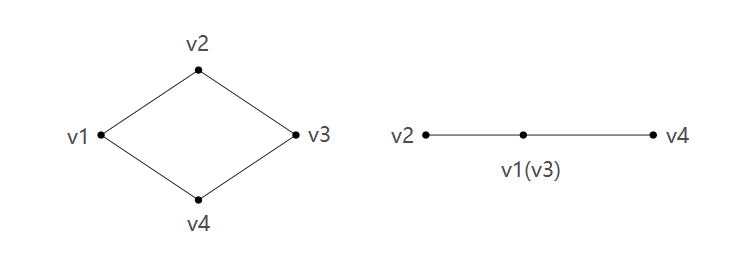
\includegraphics[width=0.5\textwidth]{figure/identifyingv1v3.png} 
\label{figure} %用于文内引用的标签
\end{figure}

\begin{block}{Reconstruction Step:}
In graph $G^{'}$, let $c_1$ be the color of $v_2$, $c_2$ be the color of $v_1$ and $c_3$ be the color of $v_4$.
\end{block}
\end{frame}

\begin{frame}{Safety of multigrams}
\framesubtitle{How to identify vertices in multigrams?}
\begin{block}{}
For \textit{hexagram} $(v_1, v_2, v_3, v_4, v_5, v_6)$, $G^{'}$ can be obtained by identifying vertices $v_1$ with $v_3$. 
\end{block}
\begin{figure}[H] %H为当前位置,!htb为忽略美学标准,htbp为浮动图形
\centering %图片居中
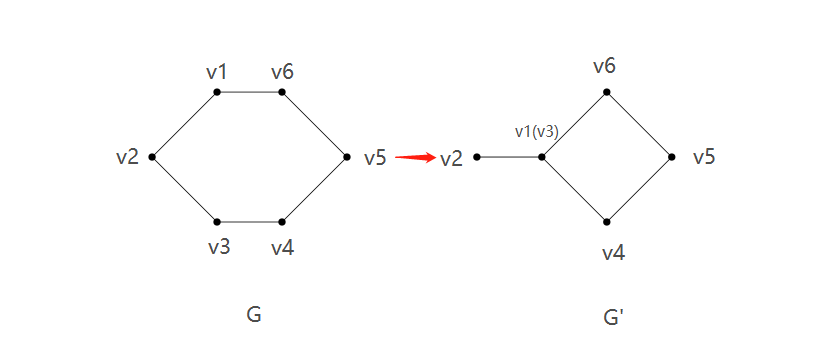
\includegraphics[width=0.6\textwidth]{figure/identifyingv1v32.png} 
\label{figure} %用于文内引用的标签

\end{figure}
\begin{block}{Reconstruction Step:}
In graph $G^{'}$, let $c_1$ be the color of $v_2$, $c_2$ be the color of $v_1$. Assume that the color of $v_4$ and $v_6$ is $c_3$ and the color of $v_5$ is $c_1$. Apparently, the color $c_2$ can be designated for $v_3$ as well.
\end{block}
\end{frame}

\begin{frame}{Safety of multigrams}
\framesubtitle{How to identify vertices in multigrams?}
\begin{block}{}
For pentagram ($v_1$, $v_2$, $v_3$, $v_4$, $v_5$), $G^{'}$ will be attained from $G \backslash \{v_1, v_2, v_3, v_4\}$ by identifying $v_5$ with $x_2$ and $x_3$ with $x_4$.
\end{block}

\begin{figure}[H] %H为当前位置,!htb为忽略美学标准,htbp为浮动图形
\centering %图片居中
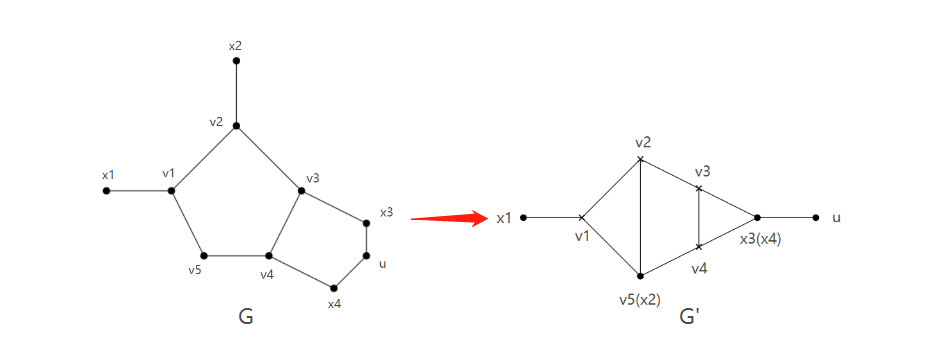
\includegraphics[width=1\textwidth]{figure/pentagramidentift.png} 
\label{figure} %用于文内引用的标签
\end{figure}

\end{frame}

\begin{frame}{Safety of multigrams}
\framesubtitle{How to identify vertices in multigrams?}
\begin{block}{Reconstruction Step:}
In graph $G^{'}$, let $c_1$ be the color of $x_1$, $c_2$ the color of $x_2$ and $v_5$, and $c_3$ the color of $x_3$ and $x_4$. Consider the following cases:
\begin{itemize}
    \item $c_1 = c_2$, we will color the remaining vertices in this order ($v_4, v_3, v_2, v_1$). Since there are at most two remaining colors when $v_i$ is colored, we can simply choose the third color for it. 
    \item $c_2 = c_3$, similarly, we will color the vertices in the reversed order as in the first case.
    \item $c_1 \ne c_2$ and $c_2 \ne c_3$, we can color $v_2$ with $c_1$, $v_1$ with $c_3$, $v_3$ with $c_2$ and $v_4$ with $c_1$.
\end{itemize}
\end{block}
\end{frame}

\begin{frame}{Demonstration}
    \begin{figure}[htbp]
\centering
\begin{minipage}[t]{0.5\textwidth}
\centering
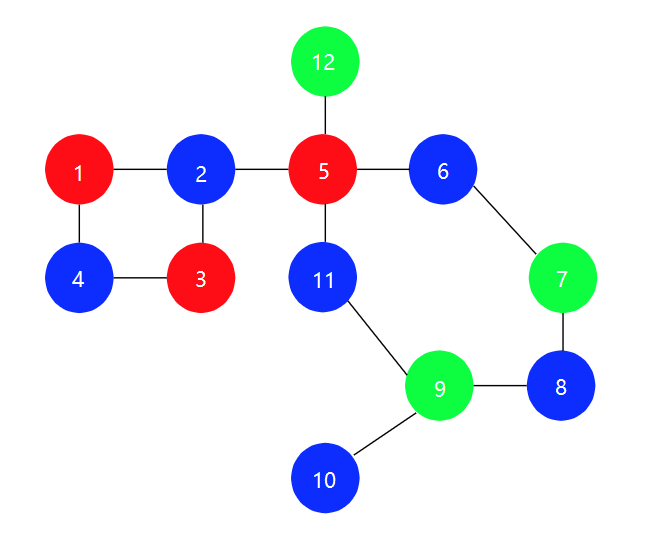
\includegraphics[width=1\textwidth]{figure/1.png}
\caption{The input graph}
\end{minipage}
\begin{minipage}[t]{0.48\textwidth}
\centering
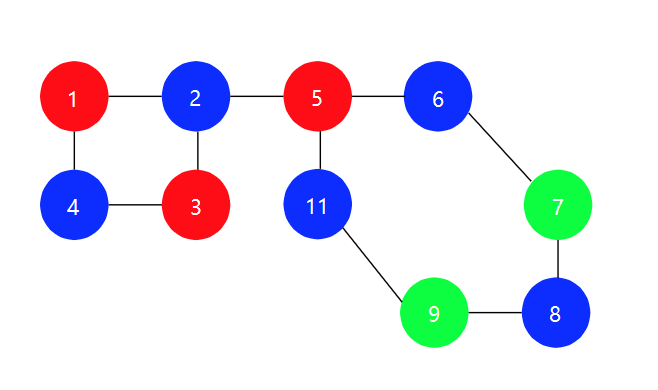
\includegraphics[width=1\textwidth]{figure/2.png}
\caption{Remove vertices with degree one}
\end{minipage}
\end{figure}
\end{frame}

\begin{frame}{Demonstration}
\begin{figure}[htbp]
\centering
\begin{minipage}[t]{0.5\textwidth}
\centering
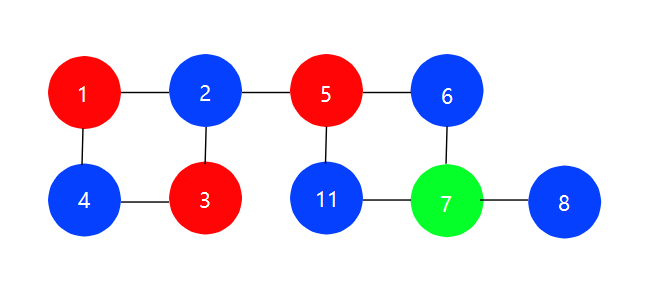
\includegraphics[width=1\textwidth]{figure/3.png}
\caption{Identify vertices 7 and 9}
\end{minipage}
\begin{minipage}[t]{0.48\textwidth}
\centering
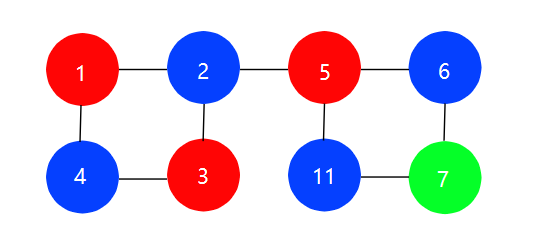
\includegraphics[width=1\textwidth]{figure/4.png}
\caption{Remove vertices with degree one}
\end{minipage}
\end{figure}
\end{frame}

\begin{frame}{Demonstration}
\begin{figure}[htbp]
\centering
\begin{minipage}[t]{0.5\textwidth}
\centering
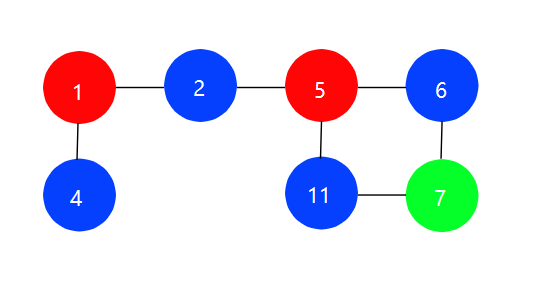
\includegraphics[width=1\textwidth]{figure/5.png}
\caption{Identify vertices 1 and 3}
\end{minipage}
\begin{minipage}[t]{0.48\textwidth}
\centering
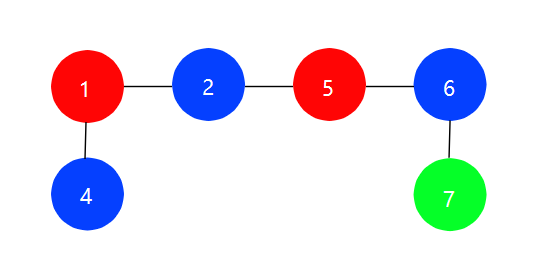
\includegraphics[width=1\textwidth]{figure/6.png}
\caption{Identify vertices 6 and 11}
\end{minipage}
\end{figure}
\end{frame}


\begin{frame}{Main argument for detecting multigrams}
    \begin{block}{Lemma 1:}
    Every triangle-free plane graph $G$ of minimum degree at least three has a safe tetragram, a safe pentagram or a safe hexagram.
    \end{block}
\end{frame}

\begin{frame}{Proof of Grötzsch's Theorem}
    \begin{block}{Grötzsch's Theorem:}
    Every triangle-free planar graph is 3-colorable.
    \end{block}
    
    \begin{block}{Proof of Grötzsch's Theorem:}
    Let $G$ as stated to be a triangle-free graph.\\
    \begin{itemize}
        \item[(1)] If there is a vertex $v$ with degree one or two, delete it. While reconstructing, give $v$ a color different from its neighbor(s).
        \item[(2)] If the minimum degree is at least three, apply Lemma 1 on the graph.
    \end{itemize}



    \end{block}
\end{frame}

\begin{frame}{Implementation}
    \begin{block}{Brute Force Algorithm:}
\begin{itemize}
    \item[(1)] Start with a vertex $v \in V$ and just go through all its adjacent vertices which should be pairwise distinct. In this step, we will use multiple inner for-loops to achieve that.
    \item[(2)] Check the condition whether the detected multigram is safe or not.
    \item[(3)] If the founded multigram is safe, then identify vertices.
    \item[(4)] Reconstruct the coloring of the graph
\end{itemize}

    \end{block}
\end{frame}

\begin{frame}{Implementation}
\framesubtitle{How to check the safety?}
\begin{block}{Testing safety:}
    \begin{itemize}
        \item Found multigram is tetragram/hexagram. We can use the same way by using two for-loops to go through all neighbors and neighbors of neighbors so that we can check that there is no path of length at most three from $v_1$ to $v_3$ which is not part of the tetragram/hexagram. This can be done in $\mathcal{O}(m^2)$ time, where $m = |E|$.
        
        \item Found multigram is pentagram. As mentioned in the former case, we can also use two for-loops to check whether there is no path in $G \backslash \{v_1, v_2, v_3, v_4\}$ of length at most three from $x_2$ to $v_5$, and every path in $G \backslash \{v_1, v_2, v_3, v_4\}$ of length at most three from $x_3$ to $x_4$ has length exactly two. This can be done in $\mathcal{O}(m^2)$ time as well.
    \end{itemize}
\end{block}
\end{frame}

\begin{frame}{Implementation - Running time analyse}
\begin{block}{Observation:}
The running time of the Brute Force algorithm is $\mathcal{O}(m^8)$ in the worst case.
\end{block}

\end{frame}





\begin{frame}{Java Implementation}
\begin{figure}[htbp]
\centering
\begin{minipage}[t]{0.48\textwidth}
\centering
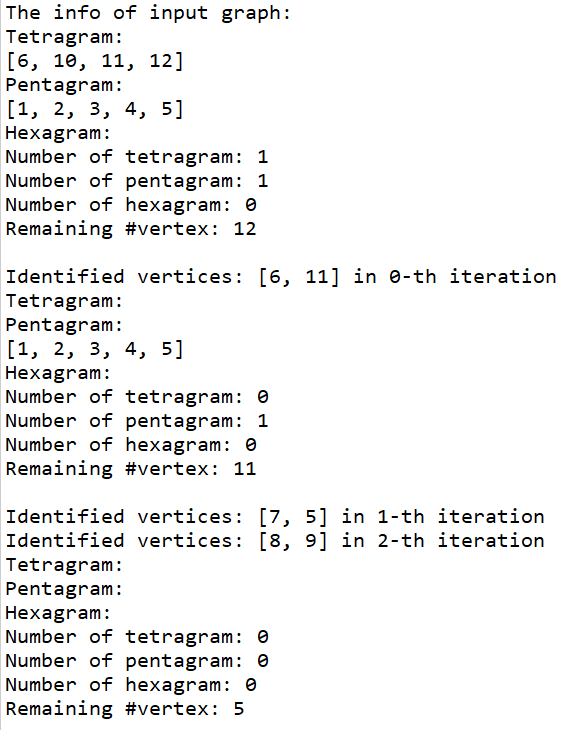
\includegraphics[width=1\textwidth]{figure/program identify.png}
\end{minipage}
\begin{minipage}[t]{0.48\textwidth}
\centering
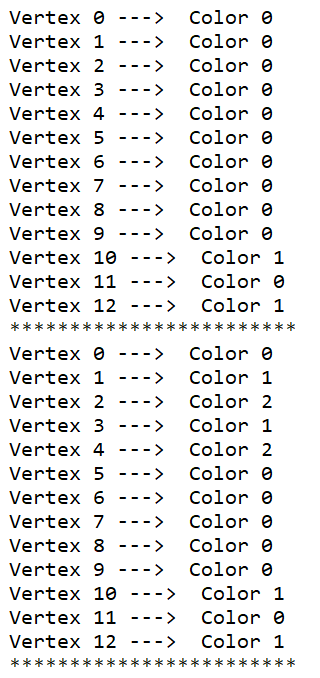
\includegraphics[width=0.6\textwidth]{figure/coloring.png}

\end{minipage}
\end{figure}
\end{frame}

\begin{frame}{Implementation - Virtualization}
    \begin{figure}[htbp]
\centering
\begin{minipage}[t]{0.48\textwidth}
\centering
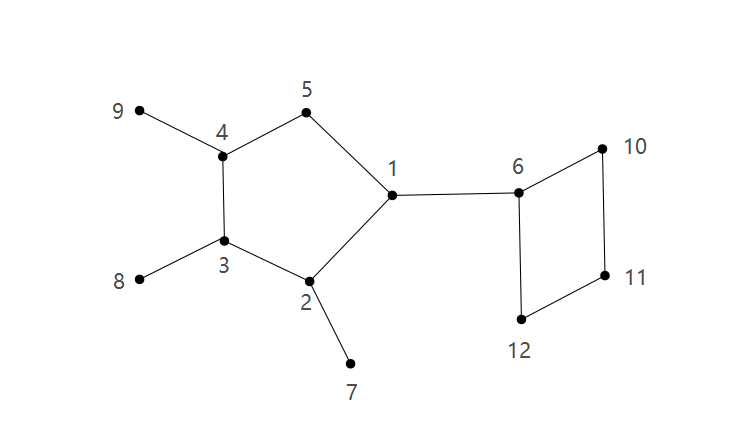
\includegraphics[width=1\textwidth]{figure/input.png}
\caption{\footnotesize The input graph}
\end{minipage}
\begin{minipage}[t]{0.48\textwidth}
\centering
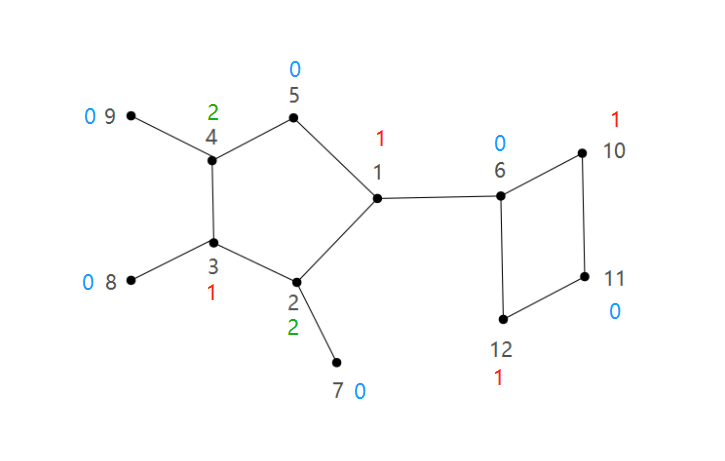
\includegraphics[width=1\textwidth]{figure/propercoloring.png}
\caption{\footnotesize The proper coloring}
\end{minipage}
\end{figure}
\end{frame}

\begin{frame}{Implementation - Improvments}
    \begin{itemize}
    \item \textbf{Tetragram.} 
\begin{itemize}
    \item[(1)] Use two loops to go through all edges $e_1, e_2 \in E$, where $e_1 \ne e_2$ and check whether they form a cycle.
    \item[(2)] Check the condition of safety by using BFS.
\end{itemize}
     The running time of this improved algorithm for detecting tetragrams is $\mathcal{O}(m^3)$.

     \item \textbf{Hexagram.} 
     \begin{itemize}
         \item[(1)]  Use three loops to go through all edges $e_1, e_2, e_3 \in E$, where $e_1 \ne e_2$ and $e_2 \ne e_3$ and check whether they form a cycle.
         \item[(2)] Check the condition of safety by using BFS analogously.
     \end{itemize}
    Totally, the running time is $\mathcal{O}(m^4)$.
\end{itemize}
\begin{figure}[htbp]
    \centering
    \begin{minipage}[t]{0.48\textwidth}
    \centering
    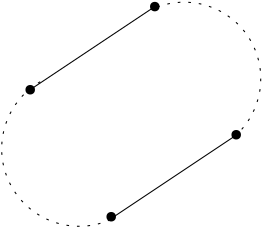
\includegraphics[width=0.5\textwidth]{figure/improve1.png}
    \end{minipage}
    \begin{minipage}[t]{0.48\textwidth}
    \centering
    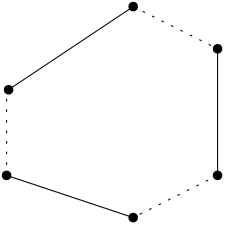
\includegraphics[width=0.5\textwidth]{figure/improve2.png}
    \end{minipage}
    \end{figure}
\end{frame}

\begin{frame}{Implementation - Improvments}
    \begin{itemize}
    \item \textbf{Pentagram.}  We use two loops to go through all edges $e_1, e_2 \in E$, where $e_1 \ne e_2$ and another loop to go through all remaining vertices. Then, we apply BFS to check wether there is a path in $G \backslash \{v_1, v_2, v_3, v_4\}$ of length at most three from $x_2$ to $v_5$ and every path in $G \backslash \{v_1, v_2, v_3, v_4\}$ of length at most three has length exactly two. Therefore, the running time is $\mathcal{O}(m^4)$. 

\end{itemize}
\begin{block}{Conclusion:}
As a result, the running time can be improved to $\mathcal{O}(m^4)$ in the worst case. 
\end{block}
\end{frame}

%\begin{frame}{Vordefinition}
%    \onslide<1,2>\begin{block}{\textbf{Definition 1:}}
%    \end{block}
%   \onslide<2>\begin{block}{\textbf{Beobachtung 2: }}
%    \end{block}
%\end{frame}

\begin{frame}{End}
    \textbf{\huge Thank you for your attention!}
\end{frame}


\end{document}
